\documentclass[border=12]{standalone}
\usepackage{tikz}
\usepackage{fixltx2e}

\usetikzlibrary{positioning,fit,calc}
\tikzstyle{train_full} = [draw=black,
						  thick,
						  text width=2cm,
						  minimum height=4cm,
						  align=center,fill=blue,
						  fill opacity=.3,
						  anchor=north east]
\tikzstyle{test_full} = [draw=black,
						 thick,
						 text width=2cm,
						 minimum height=1.4cm,
						 align=center,
						 fill opacity=0.3,
						 fill=yellow!90!black,
						 anchor=north east]
\tikzstyle{test_smally} = [draw=black,
						 thick,
						 text width=2cm,
						 minimum height=0.1cm,
						 align=center,
						 fill opacity=0.3,
						 fill=yellow!90!black,
						 anchor=north east]
\tikzstyle{train_small} = [draw=black,
						 thick,
						 text width=2cm,
						 minimum height=0.7cm,
						 align=center,
						 fill opacity=0.3,
						 fill=blue,
						 anchor=north east]
\tikzstyle{test_small} = [draw=black,
						 thick,
						 text width=2cm,
						 minimum height=0.1cm,
						 align=center,
						 fill opacity=0.3,
						 fill=blue,
						 anchor=north east]


\tikzstyle{full_data} = [draw=black,
						  thick,
						  text width=2cm,
						  minimum height=5.53cm,
						  align=center,
						  fill=green!80!black,
						  fill opacity=.3,
						  anchor=north east]

\begin{document}

    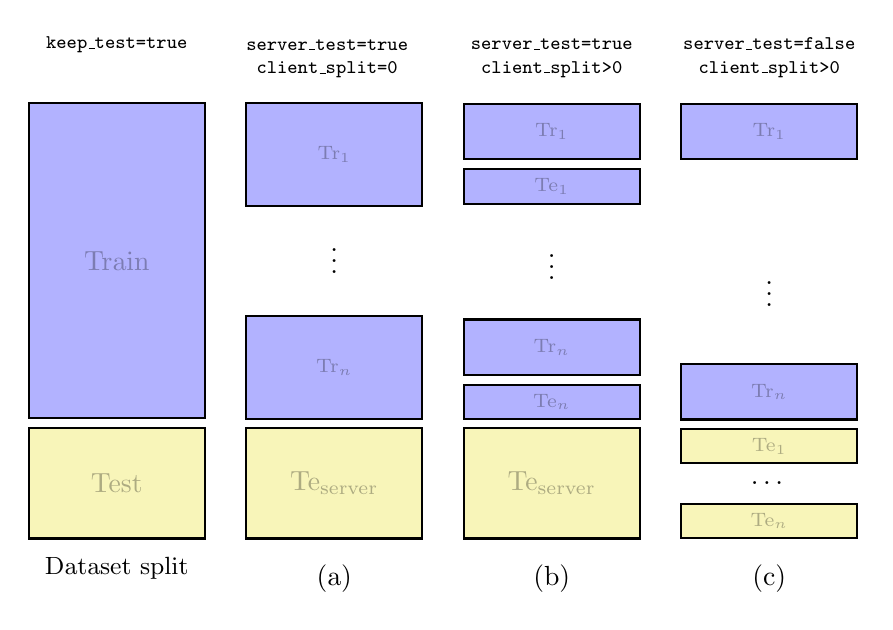
\begin{tikzpicture}
    	
        \node[train_full] (tr) {Train};
        \node[test_full, below=of tr, yshift=0.9cm] (te) {Test};
        \node[below=of te, yshift=.9cm] (label) {\small Dataset split};
        
        %%%%%%%%%%%%
        % COLUMN 1 %
        %%%%%%%%%%%%
        \node[train_small, right=of tr, xshift=-0.5cm, yshift=1.35cm, minimum height=1.3cm] (tr1) {{\scriptsize Tr$_1$}};
        \node[below=of tr1, yshift=0.8cm] (dots) {\vdots};
        \node[train_small, below=of dots, yshift=0.6cm, minimum height=1.3cm] (trn) {{\scriptsize Tr$_n$}};
        \node[test_full, right=of te, xshift=-0.5cm] (tes) {Te\textsubscript{server}};
        \node[above=of tr, yshift=-.5cm] (keeptrue) {\scriptsize \texttt{keep\_test=true}};
        \node[right=of keeptrue, xshift=-0.5cm] (stest) {\scriptsize \texttt{server\_test=true}};
        \node[below=of stest, yshift=1.1cm] (noclisplit) {\scriptsize \texttt{client\_split=0}};
		\node[below=of tes, yshift=.8cm] (label1) {(a)};        

        %%%%%%%%%%%%
        % COLUMN 2 %
        %%%%%%%%%%%%        
        \node[train_small, right=of tr1, xshift=-0.5cm, yshift=0.29cm] (tr1>0) {{\scriptsize Tr$_1$}};
        \node[test_small, below=of tr1>0, yshift=0.9cm] (te1) {{\scriptsize Te$_1$}};
        \node[below=of te1, yshift=0.7cm] (dots>0) {\vdots};
        \node[train_small, below=of dots>0, yshift=0.635cm] (trn>0) {{\scriptsize Tr$_n$}};
        \node[test_small, below=of trn>0, yshift=0.9cm] (ten) {{\scriptsize Te$_n$}};
        \node[test_full, right=of tes, xshift=-0.5cm] (tes>0) {Te\textsubscript{server}};
%        \node[above=of tr1>0] (keeptrue>0) {\scriptsize \texttt{keep\_test=true}};
        \node[above=of tr1>0, yshift=-0.45cm] (stest>0) {\scriptsize \texttt{server\_test=true}};
        \node[below=of stest>0, yshift=1.1cm] (clisplit>0) {\scriptsize \texttt{client\_split>0}};
        \node[below=of tes>0, yshift=.8cm] (label2) {(b)};
        
 		%%%%%%%%%%%%
        % COLUMN 3 %
        %%%%%%%%%%%%   
        
        
        \node[train_small, right=of tr1>0, xshift=-0.5cm] (tr1ns) {{\scriptsize Tr$_1$}};
        \node[below=of tr1ns, yshift=-0.2cm] (dotsns) {\vdots};
        \node[train_small, below=of dotsns, yshift=0.4cm] (trnns) {{\scriptsize Tr$_n$}};      
		\node[test_smally, below=of trnns, yshift=0.91cm] (te1ns) {{\scriptsize Te$_1$}};
		\node[below=of te1ns, yshift=0.9cm] (hdots) {\dots};
		\node[test_smally, below=of hdots, yshift=.9cm] (tenns) {{\scriptsize Te$_n$}};
%        \node[above=of tr1ns] (keeptrue>0) {\scriptsize \texttt{keep\_test=true}};
        \node[above=of tr1ns, yshift=-0.45cm] (stestns) {\scriptsize \texttt{server\_test=false}};
        \node[below=of stestns, yshift=1.1cm] (clisplitns) {\scriptsize \texttt{client\_split>0}};
        \node[below=of tenns, yshift=.8cm] (label3) {(c)};
                
    \end{tikzpicture}

    
\end{document}